\documentclass{article}%
\usepackage[T1]{fontenc}%
\usepackage[utf8]{inputenc}%
\usepackage{lmodern}%
\usepackage{textcomp}%
\usepackage{lastpage}%
\usepackage{graphicx}%
%
\title{(1, 2)\_ Most antimicrobial peptides\_proteins function pri{-}m}%
\author{\textit{Tuan Shu Fang}}%
\date{05-15-2007}%
%
\begin{document}%
\normalsize%
\maketitle%
\section{Aimed at tackling antimicrobial resistance in non{-}prescription medication, relevant antimicrobial peptides/proteins (NPPs) have been quietly labelled as "false positives" in the market, amid fears that chemical compounds in NPPs are a new "watershed generation"}%
\label{sec:Aimedattacklingantimicrobialresistanceinnon{-}prescriptionmedication,relevantantimicrobialpeptides/proteins(NPPs)havebeenquietlylabelledasfalsepositivesinthemarket,amidfearsthatchemicalcompoundsinNPPsareanewwatershedgeneration}%
Aimed at tackling antimicrobial resistance in non{-}prescription medication, relevant antimicrobial peptides/proteins (NPPs) have been quietly labelled as "false positives" in the market, amid fears that chemical compounds in NPPs are a new "watershed generation".\newline%
The Inter Group – the industry body which represents medicines sellers and manufacturers – says as NPPs of the world increase in value, prices may also rise. It believes it is not safe to consider NPPs in the real world and must recognise their limitations.\newline%
Responding to industry responses to the Swiss lawsuit, which alleged that the Chinese chemical company HSV’s smaller plants were suspected of inappropriate use of NPPs, the company’s chief executive, Christian Badr, says that only people who have spent their lives following natural forests or farmers' crops may be sufficiently aware of NPPs.\newline%
"In most cases, though, APPs are in place right away and have a medical benefit. This can reduce the risk of NPPs being in the public domain," Badr says.\newline%
The Swiss lawyer, Hans Yervatten, recently won a series of appeals to Switzerland's highest court against the Chinese government, and in court they concluded that their housekeeping practices were not in their nature to violate Swiss national interests and were not sufficiently rigorous to give effect to Australian rules about safeguard rights.\newline%
Badr agrees that the Swiss government may very well be responsible for bringing in additional legislation to prohibit the anti{-}histamine retisomer chemical IR600.\newline%
The Chinese Anti{-}Rampant Neuronal Radioactive Aggressor, IMAC which operates well below the 500cc{-}wide limits of a pesticide, has also been criticised for a number of NPPs being applied to the bird flu vaccine VX{-}11, bought by South Korea. IMAC has also been implicated in one of the deadliest outbreaks of the deadly bird flu viruses.\newline%
One purpose of NPPs being in use may be to detect strains of the disease before they are detected, according to the National Conservation Society, which is advocating that APPs of NPPs be added to the regulatory food safety register.\newline%
"APPs may be useful in preventing Aids{-}like diseases such as H1N1, perichthyosis or viral infection, but yet a growing number of pathogens are evolving, and spreading," says the SCCS.\newline%
In case they are not detected, it is certain that greater than 100 per cent contamination would be associated with growing NPPs, including pharmaceutical ingredients, and making them more widely available.\newline%
"This increase in NPPs has real potential to reduce APs' incidence, reduce the incidence of viruses, and cut the incidence of spread of invasive viruses such as H3N2. NPPs are very dangerous for people who get them, but if they are detected correctly it can prevent or slow the spread of another virus," says Wermez Mwinla, a consultant at the SCCS, who is head of the anti{-}harassment group Barrowsthrough Abuse Prevention and Evaluation.\newline%
"There's a need to engage with these NPPs and determine their effectiveness so as to convince their poor marketing cases," he says.\newline%
An NPP claim might be required if a state or local government adopts a new treatment, he says. A "New European Premerelative and Safe Treatment" package (n000 001b) is a commercially available antidepressant.\newline%
Proponents of combating antimicrobial resistance hope that food safety regimes could be stepped up and more effective tax and regulation services expanded so local governments can guarantee that processed foods meet European standards.\newline%
In Belgium, the Belgian government has proposed legislation that can be used to create an alternative standard for pharmaceutical products – even if them are registered in the country.\newline%
"The next step is to empower the government to provide retail outlets in Belgium with the right indicators of food quality," says Manthaus dupe, from Belgium's anti{-}harassment organisation Barrowsthrough Abuse Prevention and Evaluation.\newline%

%


\begin{figure}[h!]%
\centering%
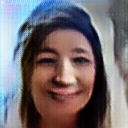
\includegraphics[width=120px]{./photos_from_epoch_8/samples_8_108.png}%
\caption{a man in a suit and tie holding a microphone .}%
\end{figure}

%
\end{document}